\documentclass[13.5pt,aspecratio=169]{beamer}
\usepackage{graphicx} % Required for inserting images
\usepackage{amsfonts}
\usepackage{amsmath}
\usepackage{amssymb}
\usepackage{physics}
\usepackage{bm}
\usepackage{physics}
\usepackage{booktabs}
\usepackage{setspace}
\usepackage{xcolor}
\usepackage{wrapfig,lipsum}
\usetheme{Madrid}
\useinnertheme{circles}

\DeclareMathOperator*{\argmax}{arg\,max}
\DeclareMathOperator*{\argmin}{arg\,min}
\graphicspath{{Images/}{./}} 
\usetheme{Copenhagen}
%\usecolortheme{beaver}
\title{CHAPTER 8: Sequence Labeling for Parts of
Speech and Named Entities}
\author[Group 5]{\textit{Instructor: PhD. Nguyen Thi Quy}\\ \bigskip \textbf{Group 5: 8.3 - 8.4.3}}
\date{\today}
\definecolor{mylightgreencolor}{RGB}{144, 238, 144}
\definecolor{mylightredcolor}{RGB}{255, 204, 203}
\setbeamertemplate{navigation symbols}{}
\setbeamertemplate{headline}{}
\setbeamercolor{huge text}{fg=white}
\setbeamertemplate{footline}{
    \leavevmode%
    \hbox{%
        \begin{beamercolorbox}[wd=.333333\paperwidth,ht=2.25ex,dp=1ex,center]{author in head/foot}%
            \usebeamerfont{author in head/foot}\insertshortauthor
        \end{beamercolorbox}%
        \begin{beamercolorbox}[wd=.333333\paperwidth,ht=2.25ex,dp=1ex,center]{title in head/foot}%
            \usebeamerfont{title in head/foot}\insertshorttitle
        \end{beamercolorbox}%
        \begin{beamercolorbox}[wd=.333333\paperwidth,ht=2.25ex,dp=1ex,right]{date in head/foot}%
            \usebeamerfont{date in head/foot}\insertshortdate{}\hspace*{2em}
            \insertframenumber{} / \inserttotalframenumber\hspace*{2ex} 
        \end{beamercolorbox}%
    }%
    \vskip0pt%
}

\begin{document}
\maketitle

% \begin{frame}
% 	\frametitle{Table of Contents} % Slide title, remove this command for no title
% 	\tableofcontents[subsectionstyle=hide]
% \end{frame}
%-------------------------------------------------------------------%


\begin{frame}
    \doublespacing
        \frametitle{Presentation Overview} % Slide title, remove this command for no title
        
        \tableofcontents % Output the table of contents (all sections on one slide)
        %\tableofcontents[pausesections] % Output the table of contents (break sections up across separate slides)
\end{frame}
    
    %----------------------------------------------------------------------------------------
    %	PRESENTATION BODY SLIDES
    %----------------------------------------------------------------------------------------
    
    \section{8.3 Named Entities and Named Entity Tagging} % Sections are added in order to organize your presentation into discrete blocks, all sections and subsections are automatically output to the table of contents as an overview of the talk but NOT output in the presentation as separate slides
    %------------------------------------------------
    \begin{frame}
        \doublespacing
            \frametitle{Presentation Overview} % Slide title, remove this command for no title
            
            \tableofcontents[currentsection] % Output the table of contents (all sections on one slide)
            %\tableofcontents[pausesections] % Output the table of contents (break sections up across separate slides)
    \end{frame}

%-------------------------------------------------------------------%


\begin{frame}
    \onehalfspacing
        \frametitle{Named Entities}
        
        \begin{block}{} % Block without title
                 {\textbf{Named entity}, in its core usage, means anything that can be referred to with a proper name. Most common 4 tags:}
                    \begin{itemize}
                        \item PER (Person): \color{blue} “Marie Curie” \color{black}
                        \item LOC (Location): \color{blue} “New York City”  \color{black}
                        \item ORG (Organization): \color{blue} “Stanford University” \color{black}
                        \item GPE (Geo-Political Entity): \color{blue} "Boulder, Colorado" \color{black}
                    \end{itemize}
        \end{block}
            \bigskip
    \end{frame}
    
    %--------------------------------------------------
    \begin{frame}
    \onehalfspacing
        \frametitle{Named Entities}
        
        \begin{block}{} % Block without title
                 
                    \begin{itemize}
                        \item Often multi-word phrases
    
                        \item But the term is also extended to things that aren't entities: dates, times, prices
                    \end{itemize}
        \end{block}
    \end{frame}
    
    
    %------------------------------------------------
    \begin{frame}
    \onehalfspacing
        \frametitle{Named Entity tagging}
        \begin{block}{The task of named entity recognition (NER):}
            \begin{itemize}
                \item Find spans of text that constitute proper names
                    \item Tag the type of the entity.          
                \end{itemize}
        \end{block}
    \end{frame}
    
    
    %------------------------------------------------
    
    
    \begin{frame}
    \onehalfspacing
        \frametitle{NER output}
        
        \begin{block}{}
            Citing high fuel prices, \color{blue}[ORG United Airlines] \color{black}said \color{blue} [TIME Friday] \color{black} it has increased fares by \color{blue} [MONEY \$ 6] \color{black} per round trip on flights to some cities also served by lower-cost carriers. \color{blue}[ORG American Airlines] \color{black}, a unit of \color{blue}[ORG AMR Corp.] \color{black}, immediately matched the move, spokesman \color{blue}[PER Tim Wagner] \color{black}said. \color{blue}[ORG United]\color{black}, a unit of \color{blue}[ORG UAL Corp.]\color{black}, said the increase took effect \color{blue}[TIME Thursday] \color{black} and applies to most routes where it competes against discount carriers, such as \color{blue}[LOC Chicago] \color{black} to \color{blue}[LOC Dallas] \color{black} and \color{blue}[ LOC Denver] \color{black}to \color{blue}[LOC San Francisco]\color{black}.
        \end{block}	
    \end{frame}
    %------------------------------------------------
    \begin{frame}
    \onehalfspacing
        \frametitle{Why NER?}	
        \begin{block}{}
            Sentiment analysis: consumer’s sentiment toward a particular company or person?
            \\  \bigskip
                 Question Answering: answer questions about an entity?
              \\  \bigskip
                 Information Extraction: Extracting facts about entities from text.
        \end{block}	
    \end{frame}
    %------------------------------------------------
    \begin{frame}
    \onehalfspacing
        \frametitle{Why NER is hard}	
        \begin{block}{Segmentation}
        \begin{itemize}
            \item In POS tagging, no segmentation problem since each word gets one tag.
                \item In NER we have to find and segment the entities!
        \end{itemize}
        \end{block}	
     \begin{block}{Type ambiguity}
         
    \color{blue} [PER Washington] \color{black} was born into slavery on the farm of James Burroughs. \color{blue}[ORG Washington] \color{black}went up 2 games to 1 in the four-game series. \\ 
    Blair arrived in \color{blue}[LOC Washington] \color{black} for what may well be his last state visit. In June, \color{blue}[GPE Washington] \color{black} passed a primary seatbelt law.
     \end{block}
    \end{frame}
    %------------------------------------------------------------------
    \begin{frame}
    \onehalfspacing
    
        \frametitle{BIO Tagging}	
        \color{blue}[PER Jane Villanueva] \color{black}of \color{blue}[ORG United]\color{black} , a unit of \color{blue}[ORG United Airlines Holding]\color{black} , said the fare applies to the \color{blue}[LOC Chicago]\color{black} route. 
    \begin{center}
    \renewcommand{\arraystretch}{0.83} % Default value: 1
        \begin{tabular}{ |c|c| } 
        \hline
        \large Words &  \large BIO Label\\ 
        \hline \small
        Jane & \small B-PER \\ \small
        Villanueva & \small I-PER \\ \small
        of & \small O \\ \small
        United & \small B-ORG \\ \small
        Airlines & I-ORG \\ \small
        Holding & I-ORG \\ \small
        discussed & O \\ \small
        the & \small O \\ \small
        Chicago & \small B-LOC \\ \small
        route & \small O \\ \small
        . & \small O \\ 
    \hline
    \end{tabular}
    \end{center}
    \end{frame}
    %------------------------------------------------------------------
    \begin{frame}
    \frametitle{BIO Tagging}	
    \vspace{-100pt}
    \hspace{10pt}
        {* B: token that begins a span \\
    \hspace{10pt} * I: tokens inside a span\\
    \hspace{10pt} * O: tokens outside of any span \\
    \hspace{10pt} * of tags (where n is entity types): \\
    \hspace{10pt} * 1 O tag, \\
    \hspace{10pt} * n B tags, \\
    \hspace{10pt} * n I tags \\
    \hspace{10pt} * total of 2n+1}
    \vspace{-150pt}
    \begin{wraptable}{r}{0cm}
        \begin{tabular}[b]{|c|c|}
        \hline
        \large Words &  \large BIO Label\\ 
        \hline \small
        Jane & \small B-PER \\ \small
        Villanueva & \small I-PER \\ \small
        of & \small O \\ \small
        United & \small B-ORG \\ \small
        Airlines & I-ORG \\ \small
        Holding & I-ORG \\ \small
        discussed & O \\ \small
        the & \small O \\ \small
        Chicago & \small B-LOC \\ \small
        route & \small O \\ \small
        . & \small O \\ 
    \hline
    \end{tabular}
    \end{wraptable} 
    
    \end{frame}
    
    %------------------------------------------------------------------
    \begin{frame}
    \onehalfspacing
    
        \frametitle{BIO Tagging variants: IO and BIOES}	
        \color{blue}[PER Jane Villanueva] \color{black}of \color{blue}[ORG United]\color{black} , a unit of \color{blue}[ORG United Airlines Holding]\color{black} , said the fare applies to the \color{blue}[LOC Chicago]\color{black} route. 
    \begin{center}
    \renewcommand{\arraystretch}{0.83} % Default value: 1
        \begin{tabular}{ |c|c|c|c| } 
        \hline
        \large Words &  \large IO Label & \large BIO Label & \large BIOES Label \\
        \hline \small
        Jane & \small I-PER &\small  B-PER &\small  B-PER \\  \small
        Villanueva & \small I-PER &\small  I-PER &\textbf{} E-PER \\  \small
        of & \small O &\small  O &\small  O\\  \small
        United & \small I-ORG &\small  B-ORG &\small  B-ORG \\  \small
        Airlines & \small I-ORG & I\small -ORG &\small  I-ORG \\  \small
        Holding & \small I-ORG &\small  I-ORG &\small  E-ORG \\  \small
        discussed & \small O &\small  O &\small  O\\  \small
        the & \small O &\small  O &\small  O\\  \small
        Chicago & \small I-LOC &\small  B-LOC &\small  S-LOC \\  \small
        route & \small O &\small  O &\small  O\\  \small
        . & \small O & \small O & \small O \\
    \hline
    \end{tabular}
    \end{center}
    \end{frame}
    %------------------------------------------------------------------
    \begin{frame}
    \onehalfspacing
    
        \frametitle{Standard algorithms for NER}	
        \begin{block}{}
         \large   Supervised Machine Learning given a human-labeled training set of text annotated with tags
        \begin{itemize}
            \item Hidden Markov Models
            \item Conditional Random Fields (CRF)/ Maximum Entropy Markov Models (MEMM)
            \item Neural sequence models (RNNs or Transformers)
            \item Large Language Models (like BERT), finetuned
        \end{itemize}
        \end{block}
    \end{frame}

\section{8.4 HMM Part-of-Speech Tagging} % Sections are added in order to organize your presentation into discrete blocks, all sections and subsections are automatically output to the table of contents as an overview of the talk but NOT output in the presentation as separate slides
\begin{frame}
	\frametitle{Presentation Overview} % Slide title, remove this command for no title
	\tableofcontents[currentsection]
\end{frame}

%------------------------------------------------
% {
% \begin{frame}
% 	\frametitle{Methods for POS Tagging and NER}
%     \setbeamertemplate{footline}{boo \insertframenumber}
%     \begin{minipage}{0.5\textwidth}  % Adjust the width as needed
%         {
%         \setbeamercolor{block body}{bg=mylightgreencolor} % Block body color
%         \begin{block}{} % Block without title
%             HMM – Hidden Markov chains
%         \end{block}
%         }
%         \begin{block}{} % Block without title
%             CRF – Conditional Random Fields
%         \end{block}
        
%     \end{minipage}\hspace{10pt}
%     \begin{minipage}{0.45\textwidth}  % Adjust the width as needed
%             \centering
%             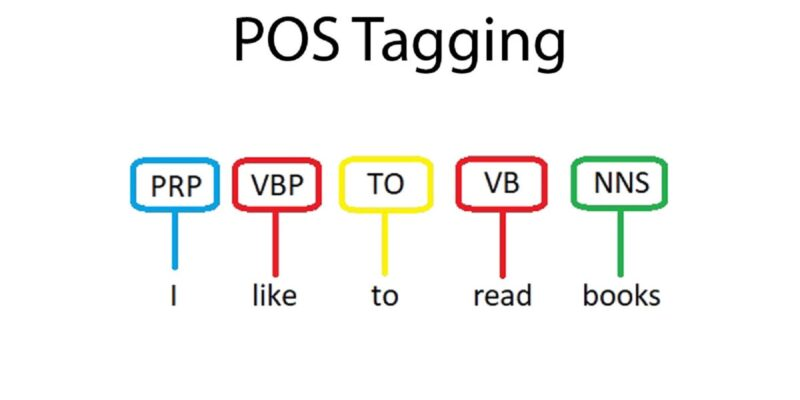
\includegraphics[scale=0.3]{POS-Tagging.jpg}
%     \end{minipage}
	
    
% \end{frame}
% }

%------------------------------------------------
\subsection{8.4.1 Markov Chains}

\begin{frame}
    \onehalfspacing
        \frametitle{Introducing HMM}
        
        \begin{block}{The Hidden Markov Model - HMM}
            \begin{itemize}
                \item A statistical model with unknown parameters that must be determined from known parameters.
                \item Extends from the mathematical model: \textbf{Markov Chains}.
            \end{itemize}
        \end{block}

        {
            \setbeamercolor{block title}{bg=mylightgreencolor, fg=black} % Block title color
            \begin{block}{Applications}
                \begin{minipage}{0.45\textwidth}
                    \begin{itemize}
                        \item Sequence labeling: NER, POS tagging
                        \item Speech recognition
                    \end{itemize}
                \end{minipage}
                \begin{minipage}{0.45\textwidth}
                    \begin{itemize}
                        \item Optical Character Recognition (OCR)
                        \item Bioinformatics
                    \end{itemize}
                \end{minipage}
            \end{block}
        }
\end{frame}
    
%------------------------------------------------

\begin{frame}
    \onehalfspacing
        \frametitle{Markov chains}
    \begin{minipage}{0.62\textwidth}

        \begin{block}{Markov chains}
            A model that tells us something about the probabilities of sequences of random variables, states
        \end{block}

        \begin{itemize}
            \item Sequence of states with a temporal order
            \item States can take values from any discrete set of values.
            \item \textbf{Markov assumption}:
            When predicting the future, the past doesn’t matter
        \end{itemize}
        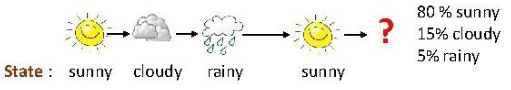
\includegraphics[width=1\textwidth]{Rain_Prediction.png}
    \end{minipage}
    \begin{minipage}{0.3\textwidth}
        \begin{figure}
            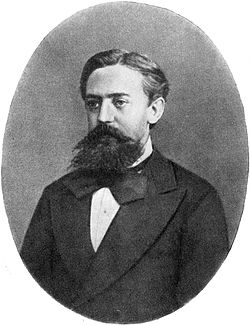
\includegraphics[scale=0.5]{AAMarkov.jpg}
            \caption{AA. Markov}
        \end{figure}
        
    \end{minipage}
        
\end{frame}

%------------------------------------------------


\begin{frame}
\onehalfspacing
	\frametitle{Markov assumption}
    {\large When predicting the future, the past doesn’t matter, only the present} \vspace{2em}

    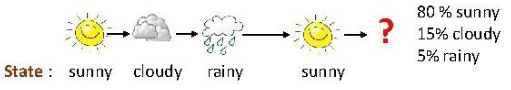
\includegraphics[width=0.62\textwidth]{Rain_Prediction.png}

    \begin{center}
        \textbf{Markov assumption}: \hspace{1em} $P(q_i = a | q_1 ... q_{i-1}) = P(q_1 = a | q_{i-1})$
    \end{center}
\end{frame}

%------------------------------------------------
\begin{frame}
    \onehalfspacing
        \frametitle{Markov chains}
        
        \begin{block}{Components of the Markov chains}
            \begin{itemize}
                \item $Q = q_1 q_2 ... q_n$: a set of N \textbf{states}
                \item $A = a_{11} a_{12} ... a_{N1} ... a_{NN}$: a \textbf{transition probability matrix} A, each $a_{ij}$ representing the probability of moving from state $i$ to state $j$
                \item $\pi = \pi_1, \pi_2,...,\pi_n$:  an \textbf{initial probability distribution} over states. $\pi_i$ is the
                probability that the Markov chain will start in state $i$.
            \end{itemize}
        \end{block}
        
\end{frame}
%------------------------------------------------
\begin{frame}
    \onehalfspacing
        \frametitle{Markov chains}
        
        \begin{minipage}{0.5\textwidth}
            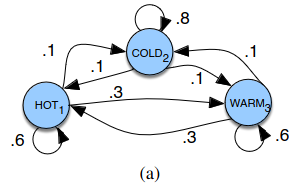
\includegraphics[scale=0.7]{Example_1.png}
        \end{minipage}
        \begin{minipage}{0.49\textwidth}
            \begin{block}{}
                Markov Chain in Figure (a)
            \end{block}

            \begin{itemize}
                \item $\textcolor{red}{Q} = \{HOT, COLD, WARM \} $ 
                \item Transition probability matrix \textcolor{red}{A}: 
                \hspace*{-1cm}
                {
                \small
                \begin{tabular}{c|cccc}
                    $ $ & $\pi$ & HOT & COLD & WARM \\
                    \hline
                    HOT & 0.7 & 0.6 & 0.1 & 0.3 \\
                    COLD & 0.1 & 0.3 & 0.8 & 0.1\\
                    WARM & 0.2 & 0.3 & 0.1 & 0.6 \\
                \end{tabular}
                }
                \item Initial probability distribution $\textcolor{red}{\pi} = [0.7,0.1,0.2]$
                
            \end{itemize}

        \end{minipage}
        
\end{frame}
%------------------------------------------------

\begin{frame}
    \onehalfspacing
        \frametitle{Markov chains}
        
        \begin{minipage}{0.5\textwidth}
            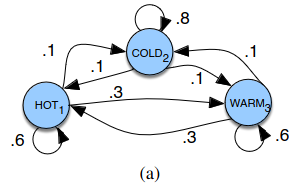
\includegraphics[scale=0.7]{Example_1.png}

            {
            \setbeamercolor{block title}{bg=mylightredcolor, fg=black} % Block title color
            \begin{minipage}{0.85\textwidth}
            \begin{block}{Calculate the probabilities of}
                \begin{enumerate}
                    \item hot hot hot hot
                    \item cold hot cold hot
                \end{enumerate}
            \end{block}
            \end{minipage}

            }
        \end{minipage}
        \begin{minipage}{0.49\textwidth}
            \begin{block}{}
                Markov Chain in Figure (a)
            \end{block}

            \begin{itemize}
                \item $\textcolor{red}{Q} = \{HOT, COLD, WARM \} $ 
                \item Transition probability matrix \textcolor{red}{A}: 
                \hspace*{-1cm}
                {
                \small
                \begin{tabular}{c|cccc}
                    $ $ & $\pi$ & HOT & COLD & WARM \\
                    \hline
                    HOT & 0.1 & 0.6 & 0.1 & 0.3 \\
                    COLD & 0.7 & 0.1 & 0.8 & 0.1\\
                    WARM & 0.2 & 0.3 & 0.1 & 0.6 \\
                \end{tabular}
                }
                \item Initial probability distribution $\textcolor{red}{\pi} = [0.1,0.7,0.2]$
                
            \end{itemize}

        \end{minipage}
        
\end{frame}
%------------------------------------------------
\subsection{8.4.2 The Hidden Markov Model}

\begin{frame}
\onehalfspacing
	\frametitle{The Hidden Markov Model}
        \begin{block}{}
            A hidden Markov model (HMM) allows us to talk about both observed events and hidden events.
        \end{block}

        {\large{Unobservable Events:}
        \begin{itemize}
            \item Part-of-speech
            \item Entity type
        \end{itemize}   
        }
        \begin{figure}
            \centering
            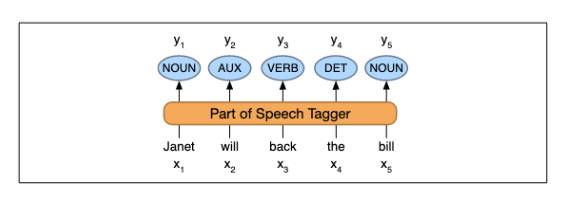
\includegraphics [scale=0.7] {POS_Tagger.png}
        \end{figure}
	
\end{frame}
%------------------------------------------------

\begin{frame}
    \onehalfspacing
        \frametitle{The Hidden Markov Model}
            \begin{figure}[h]
                \centering
                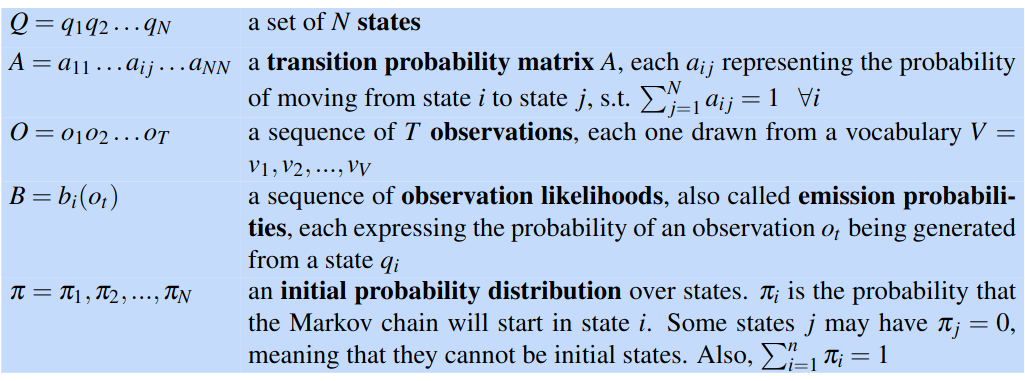
\includegraphics[scale=0.45]{HMM_components.png}
                \caption{ Components of Hidden Markov Model}
            \end{figure}
        
    \end{frame}
    %------------------------------------------------


\begin{frame}
    \onehalfspacing
        \frametitle{First order Hidden Markov Model}
        \begin{block}{A first-order HMM instantiates two simplifying assumptions}
            \begin{enumerate}
                \item The probability of a particular state depends
                only on the previous state
                \begin{center}
                    \textbf{Markov Assumption:} \hspace{0.5em} $P(q_i | q_1,...q_{i-1}) = P(q_i | q_{i-1})$
                \end{center}
                \item The probability of an output observation depends only on the state that
                produced it and not on any other states.
                \begin{center}
                    \textbf{Independence:} $P(o_i | q_1,...q_i,...,q_T, o_1,...o_i,...,o_T) = P(o_i | q_i)$
                \end{center}
            \end{enumerate}
        \end{block}
        
    \end{frame}
%------------------------------------------------
\begin{frame}
    \onehalfspacing
        \frametitle{The Hidden Markov Model}
        {
        \setbeamercolor{block title}{bg=mylightgreencolor, fg=black} % Block title color
        \begin{block}{ A sample HMM for the ice cream task. }
            \begin{itemize}
                \item The two hidden states
                (H and C) correspond to \textbf{hot} and \textbf{cold} weather,
                \item The observations $O = {1,2,3}$: number of ice creams eaten by Jason on a
                given day
            \end{itemize}
        \end{block}
    }

    \begin{figure}[h]
        \centering
        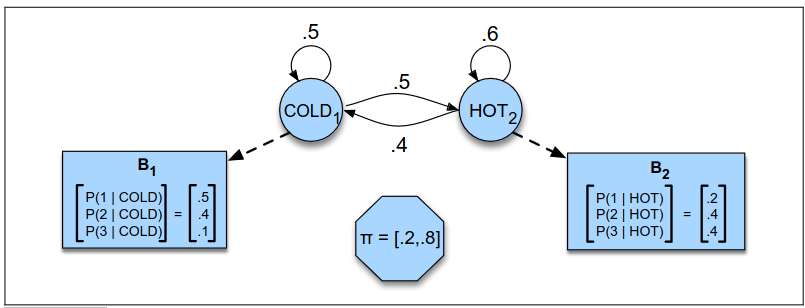
\includegraphics[scale=0.45]{HMM_ice_example.png}
        \caption{A hidden Markov model for relating numbers of ice creams eaten by Jason (the
        observations) to the weather (H or C, the hidden variables).}
    \end{figure}
    \end{frame}
%------------------------------------------------

\subsection{8.4.3 The components of an HMM tagger}
\begin{frame}
    \onehalfspacing
        \frametitle{HMM Tagger}
        \begin{block}{}
            A model in Natural Language Processing based on HMM, used for labeling elements in a sequence.
        \end{block}
        HMM Tagger consists of 2 components:
        \begin{enumerate}
            \item A: The probability of a tag occurring given the previous tag
            \item B: The probability, given a tag, that it will be associated with a given word
        \end{enumerate}
    \end{frame}
%------------------------------------------------
\begin{frame}
\onehalfspacing
	\frametitle{HMM Tagger}
    {\Large The probability of a tag occurring given the previous tag
    \begin{center}
        $P(t_i | t_{i-1}) = \dfrac{C(t_{i-1}, t_i)}{C(t_{i-1})}$
    \end{center}}

    {
        \setbeamercolor{block title}{bg=mylightgreencolor, fg=black} % Block title color
        \begin{block}{Example - In the WSJ corpus:}
            \begin{itemize}
                \item MD occurs \textbf{13124} times
                \item MD is followed
                by VB \textbf{10471} times
            \end{itemize}
            Tag transition probability MD - VB:
            \begin{center}
                $ P(VB | MD) = \dfrac{C(MD, VB)}{C(MD)} = \dfrac{10471}{13124} = 0.8 $
            \end{center}
        \end{block}
    }
\end{frame}

%------------------------------------------------
\begin{frame}
    \onehalfspacing
        \frametitle{HMM Tagger}
        {\Large The probability of a word occurring associated with a tag
        \begin{center}
            $P(w_i | t_i) = \dfrac{C(t_i, w_i)}{C(t_i)}$
        \end{center}}
    
        {
            \setbeamercolor{block title}{bg=mylightgreencolor, fg=black} % Block title color
            \begin{block}{Example - In the WSJ corpus:}
                \begin{itemize}
                    \item MD occurs \textbf{13124} times
                    \item MD is associated
                    with \textit{will} \textbf{4046} times
                \end{itemize}
                Tag transition probability MD - VB:
                \begin{center}
                    $ P(will | MD) = \dfrac{C(MD, will)}{C(MD)} = \dfrac{4046}{13124} = 0.31 $
                \end{center}
            \end{block}
        }
    \end{frame}

%------------------------------------------------


\onehalfspacing
\begin{frame} % Use [allowframebreaks] to allow automatic splitting across slides if the content is too long
	\frametitle{Reference}
	
	\begin{thebibliography}{99} % Beamer does not support BibTeX so references must be inserted manually as below, you may need to use multiple columns and/or reduce the font size further if you have many references
		\footnotesize % Reduce the font size in the bibliography
		
		\bibitem[Stanford]{p1}
			Speech and Language Processing (3rd ed. draft)
			\newblock Dan Jurafsky and James H. Martin
			\newblock Part I: Fundamental Algorithms, \emph{Chapter 8: Sequence Labeling for Parts of
            Speech and Named Entities}
			
	\end{thebibliography}
\end{frame}



%	CLOSING SLIDE
%----------------------------------------------------------------------------------------

\begin{frame} % The optional argument 'plain' hides the headline and footline
	\begin{center}
		{\Huge Thanks for listening!}
		
		\bigskip\bigskip % Vertical whitespace
		
		{\LARGE Q\&A section}
	\end{center}
\end{frame}
%------------------------------------------------


\end{document}
